\documentclass{article}
\usepackage[utf8]{inputenc}
\usepackage{fancyhdr}
\usepackage[hidelinks]{hyperref}
\usepackage[ngerman]{babel}
\usepackage{graphicx}
\usepackage{wrapfig}

\graphicspath{ ../img/ }

%\usepackage{hyperref}
%\usepackage{titling}

%\newcommand{\subtitle}[1]{
%\posttitle{
%\par\end{center}
%\begin{center}\LARGE#1\end{center}
%\vskip0.5em}
%}

\title{\textbf{\LARGE 3D-VIDEO MIT H.264/MVC
\\{\Large Technische Universit\"at Dresden}
\\\noindent\newline{\large Hauptseminar Betriebssysteme}
\\{\small Professur f\"ur Betriebssysteme}
}}
%\subtitle{Pseudozuffalsfolgengeneratoren}

%\title{\LARGE Pseudozuffalsfolgengeneratoren}
\author{\\ \Large Jan Schultke}
\date{\large2019-11-22}

\pagestyle{fancy}
\fancyhf{}
\rhead{\nouppercase{\leftmark}}
\lhead{3D-VIDEO MIT H.264/MVC}
%\rfoot{Page \thepage}
\cfoot{\thepage}

\setcounter{tocdepth}{3}
%\renewcommand{\footrulewidth}{0.5pt}
\renewcommand\refname{9 Literaturverzeichnis}
\renewcommand{\contentsname}{Inhaltsverzeichnis}
%\parskip = \baselineskip

\renewcommand{\figurename}{Abbildung }

\begin{document}

    %\section{Title}\label{sec:title}
    \maketitle
    \pagenumbering{gobble}
    \clearpage
    \pagebreak

    \pagenumbering{arabic}
    \tableofcontents
    \clearpage
    \pagebreak

    \section{Einleitung}\label{sec:intro}
    B\"ucher, Filme, Spiele: wir haben zahlreiche Wege in andere Welten abzutauchen.
Doch die wenigsten dieser Mittel haben die Mach uns wahrhaft in ihren Bann zu rei{\ss}en, uns einen kalten Schauer \"uber
den R\"ucken zu jagen, uns das Gef\"uhl zu geben, man w\"are wirklich in einer anderen Welt.
Eines dieser Mittel ist der Film, besser noch im Kino und am besten in 3D.
Der erste 3D-Film in einem IMAX-Kino ist schlichtweg unvergesslich.

\begin{center}
    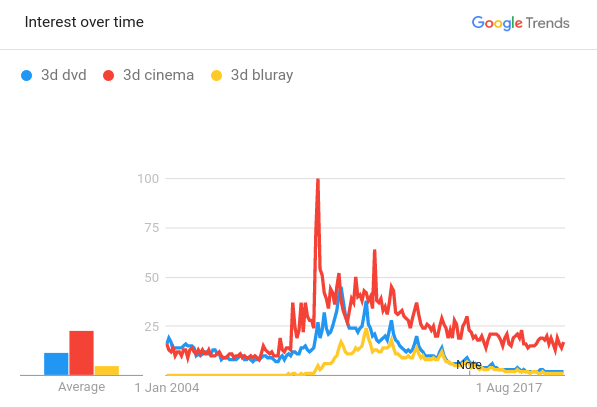
\includegraphics[width=0.66\textwidth]{../img/trends-3d.png}
\end{center}
\noindent\\ Dieses unvergessliche Erlebnis ins eigene Zuhause zu bringen bewegte viele Menschen ihr Heimkino mit 3D-Technologie
auszur\"usten.
3D-Fernseher, 3D-Blu-Ray Player, usw.
Zwar ist dieser 3D-Hype inzwischen recht abgeklungen (siehe Diagramm), doch die Technologien dahinter -insbesondere
das Kodieren mehrerer Ansichten in nur einem Datenstrom (\textit{Multi-View-Coding} oder \texttt{MVC})- sind nach wie
vor
relevant.

\noindent\\ Ein Filmstudio kann zum Beispiel noch beim Schneiden 3D-Effekte probeweise per \texttt{MVC} kodieren,
bevor der Film dann unkomprimiert an das Kino gereicht wird.
Auch im Bereich \"Uberwachung kann stark vom effizienten Kodieren mehrerer Ansichten profitiert werden.
Immerhin befinden sich schlie{\ss}lich mehr als eine Kamera an vielen \"offentlichen Pl\"atzen.

\noindent\\ Die folgende Ausarbeitung pr\"asentiert, wie dreidimensionale Videos entstehen, wahrgenommen werden und
effizient mithilfe von \texttt{H.264} kodiert werden k\"onnen.
Begleitend dazu existiert eine Web-Präsentation als Git-Repository\cite{github}.


    \pagebreak

    \section{Problem}\label{sec:problem}
    Das parallele Kodieren von zwei oder mehreren Ansichten bringt zweierlei Herausforderungen mit sich:
\begin{itemize}
    \item Komprimieren des Datenstroms durch Ausnutzen von Redundanz zwischen \"ahnlichen Perspektiven
    \item Multiplexing der Rahmen unterschiedlicher Perspektiven in einen einzigen, kontinuierlichen Datenstrom
\end{itemize}

\noindent Mit \texttt{H.264} l\"asst sich zumindest der zweite Punkt \textbf{naiv} mithilfe von \textit{Simulcast}\cite{
simulcast} bew\"altigen.
Hierbei werden mehrere Ansichten unabh\"angig voneinander kodiert und dekodiert.
Redundanzen zwischen den Perspektiven bleiben unausgenutzt, der Aufpreis pro Perspektive ist somit im
Durchschnitt 100\%.
Unser Kompressionsverfahren muss von daher einen geringeren Aufpreis haben um seine Anwendung zu rechtfertigen.


    \pagebreak

    \section{Related Work}\label{sec:relwork}
    Die Implementierung von effizienter \texttt{MVC}-Kodierung basiert gr\"o{\ss}tenteils auf
\textit{Efficient Compression of Multi-View Video Exploiting Inter-View Dependencies Based on \texttt{H.264/MPEG4-AVC}}
von P. Merkle, K. M\"uller, A. Smolic, und T. Wiegand~\cite{paper}.
Dabei handelt es sich um eines von mehreren Papieren, welches noch vor der Standardisierung 2009~\cite{mvc} von
\texttt{MVC} in \texttt{H.264} als Vorschlag f\"ur eine solche Kodierung ver\"offentlich wurde.

\noindent\\ Der H.264-Standard selbst~\cite{h264}, welcher in der aktuellen Ausgabe kostenpflichtig verf\"ugbar ist, beschreibt
lediglich die allgemeine Struktur des \texttt{H.264}-Datenformats.
Dazu z\"ahlen die Arten und Abfolgen von Rahmen, die Gr\"o{\ss}e von Macrobl\"ocken
(siehe~[\texttt{\nameref{subsec:h.264}}]), Header-Information am Anfang eines Rahmens und vieles mehr.
Die konkrete Abfolge von Rahmen, wie z.B. die oft verwendete \texttt{IBBBPBBBPBPI}-Abfolge\cite{frame-order} steht
hingegen dem Kodierer frei zur Wahl.

\noindent\\ Am 29.10.2019 wurde \texttt{FRIM 1.00}~\cite{frim} ver\"offentlicht.
Hierbei handelt es sich um einen Encoder und Decoder f\"ur \texttt{H.264} mit \texttt{MVC}, welcher f\"ur
Microsoft Windows (x86/x86\_64) verf\"ugbar ist.
Zum Experimentieren mit 3D-Videos ist dieser ein sehr geeignetes und vor allem kostenloses Werkzeug.

\noindent\\ \texttt{MVC} wird bedauernswerterweise nicht vom popul\"aren Kommandozeilenprogramm
\texttt{ffmpeg}~\cite{ffmpeg} unterst\"utzt.
So werden zus\"atzliche Ansichten beim Dekodieren schlichtweg ignoriert.



    \pagebreak

    \section{Grundlagen}\label{sec:basics}
    \subsection{Tiefenwahrnehmung des Menschen}\label{subsec:depth-percept}
Um zu verstehen, wie 3D-Medien kodiert werden k\"onnen, ist es zun\"achst wichtig zu verstehen, wie die Tiefenwahrnehmung
beim Menschen funktioniert.
Wir unterscheiden zwischen \textit{monokularen} und \textit{binokularen} Faktoren.
Monokulare Faktoren sind von nur einer Perspektive (Auge oder Kameralinse) abh\"angig.
Dazu z\"ahlen unter anderem\cite{depth-perception}:
\begin{itemize}
    \item Bewegungsparallaxe
    \item absolute/relative/vertraute Gr\"oße
    \item Verdeckung naher Objekte durch ferne Objekte
    \item Wahrnehmung dreidimensionaler Form durch Licht und Schatten
    \item Tiefensch\"arfe
\end{itemize}
Diese Effekte sind allesamt in nur einem einzelnen Datenstrom enkodierbar und essentiell f\"ur ein immersives Bild.

\noindent\newline Mehrere Datenstr\"ome werden hingegen f\"ur binokulare Faktoren ben\"otigt.
Hierzu z\"ahlt die Parallaxe zwischen dem linken und dem rechten Auge, sprich der Unterschied dieser zwei Perspektiven.
Objekte die hierbei n\"aher zum Betrachter liegen, werden unterschiedlicher von den Augen wahrgenommen, weiter entferntere
Objekte hingegen \"ahnlicher.
Dieser Faktor erlaubt eine \textit{echte} Tiefenwahrnehmung bis zu 10m.\cite{depth-perception}
Weiterhin wird Tiefe durch die Konvergenz der Blickachsen des Betrachters wahrgenommen.
Um besonders nahe gelegene Objekte zu betrachten, muss der Mensch seine Augen leicht nach innen drehen um das Objekt
scharf zu sehen, was dem Gehirn wiederhin erm\"oglicht, Tiefe aus dieser Konvergenz zu interpretieren.

\noindent\newline Da das \"Andern der Blickachsen eines Zuschauers ohne Gewalt nicht m\"oglich ist, bleibt somit die
Parallaxe der entscheidende, zu reproduzierende Faktor um Videos mit 3D-Effekt zu erzeugen.


\subsection{Begriffskl\"arungen zum Thema Video}\label{subsec:video-terms}
\subsubsection{Codec}
Der Begriff Codec setzt sich aus den englischen W\"ortern \textbf{co}der (Kodierer) / \textbf{dec}oder (Dekodierer)
zusammen\cite{codec} und ist ein Algorithmenpaar bestehend aus den genannten Teilen.
Er wird jedoch vor allem im Themenbereich Medien eingesetzt um Audio- und Videostandards wie \texttt{H.264} zu
bezeichnen.

\noindent\newline So ist z.B. \texttt{H.264/AVC} ein Codec, \texttt{MP4} hingegen ein Containerformat, sprich ein Dateiformat welches
die kodierten Datenstr\"ome eines Codecs enth\"alt.

\noindent\newline Die Begriffe \textit{encoder} und \textit{decoder} hingegen werden f\"ur konkrete Programme zum
Kodieren oder Dekodieren der Datenstr\"ome eines Codecs verwendet.
So ist z.B. \textt{x264}\cite{x264} ein \textit{encoder} f\"ur den Codec \texttt{H.264}

\subsection{H.264}\label{subsec:h.264}
H.264 ist ein Codec, welcher 2003\cite{h264} durch die VCEG (\textit{Video Coding Experts Group}) und MPEG
(\textit{Moving Pictures Expert Group}) als \textit{MPEG Part 10} standardisiert wurde.
Er wird auch als AVC (\textit{Advanced Video Codec}) bezeichnet.

\noindent\newline H.264 unterst\"utzt sowohl \textit{Intra-Frame-Kompression}, die Kompression von Daten innerhalb eines Rahmens sowie
\textit{Inter-Frame-Kompression}, die Kompression zwischen mehreren Rahmen.

\noindent\newline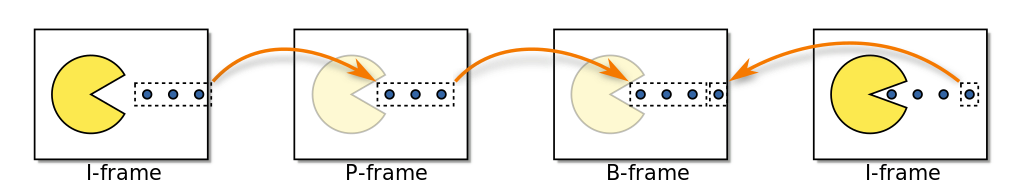
\includegraphics[width=\textwidth]{../img/frames}

\noindent\newline Kompression von Videodaten erfolgt in sogenannten \textit{Macrobl\"ocken}.
Hierbei handelt is sich um 4x4 bis 16x16 gro{\ss}e Bl\"ocke von Pixeln.

%\paragraph{Outline}
%\section*{8 Literaturverzeichnis}\label{sec:bibliography}
%Section~\ref{sec:previous work} gives account of previous work.
%Our new and exciting results are described in Section~\ref{sec:results}.
%Finally, Section~\ref{sec:conclusions} gives the conclusions.
%    \section{Previous work}\label{sec:previous work}
%    A much longer \LaTeXe{} example was written by Gil~\cite{Gil:02}.



    \pagebreak

    \section{Kernidee}\label{sec:idea}
    \subsection{Multi-View-Coding}\label{subsec:mvc}

\subsubsection{R\"aumliche und Zeitliche Nachbarn eines Rahmens}
\begin{wrapfigure}{r}{0.4\textwidth}
    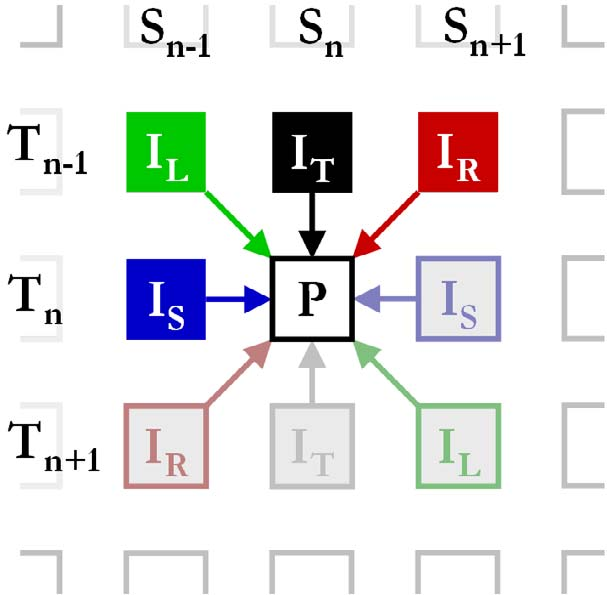
\includegraphics[width=5cm]{../img/prediction}
\end{wrapfigure}

Jeder Rahmen hat drei einzigartige r\"aumliche sowie zeitliche Nachbarn.\cite{paper}
Diese bestehen aus dem Rahmen der benachbarten Perspektive, dem vorherigen Rahmen der selben Perspektive, sowie
dem vorherigen Rahmen der benachbarten Perspektive.

\noindent\newline Es stellt sich f\"ur uns die Frage, welche der Perspektiven der beste Pr\"adiktor unseres Rahmens ist.
Durch eine statistische Analyse der mehrerer Videosequenzen kann diese Frage beantwortet werden.
Hierzu m\"ussen die Kosten des Erstellens eines P-Rahmens zwischen den Nachbarn verglichen werden.
Zwar gibt es starke Variationen zwischen Videosequenzen, im Durchschnitt ist jedoch der direkte zeitliche Nachbar
der beste Pr\"adiktor.\cite{paper}
Gefolgt wird dieser vom direkten r\"aumlichen Nachbarn.


    \pagebreak

    \section{Details eines Aspekts / Implementierung}\label{sec:impl}
    \subsection{Hierarchische Baumstrukturen}\label{subsec:htrees}

\begin{center}
    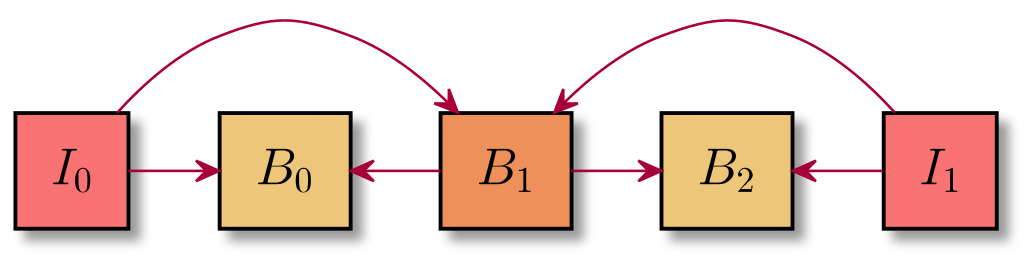
\includegraphics[width=0.75\textwidth]{../img/b-pictures}
\end{center}

Um mehrere Ansichten zu Kodieren, verwenden wir hierarchische Baumstrukturen von B-Rahmen.
Wie im Bild zu sehen, werden hier zun\"achst B-Rahmen aus Paaren von I-Rahmen erzeugt und daraus weitere B-Rahmen, usw.


\subsubsection{Hierarchische Baumstruktur f\"ur mehrere Ansichten}
\begin{center}
    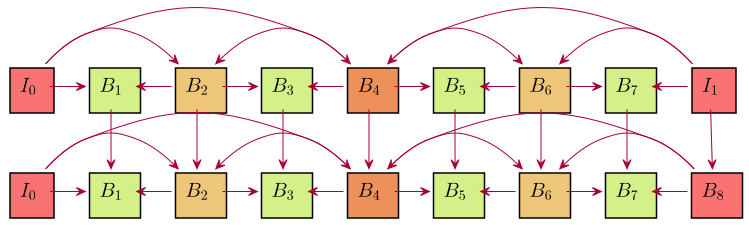
\includegraphics[width=1\textwidth]{../img/b-pictures-3d}
\end{center}
Aus diesen Ergebnissen k\"onnen wir schlussfolgern, dass unsere Kodierungsstruktur sowohl r\"aumliche als auch zeitliche
Nachbarn zum Produzieren eines B-Rahmens verwenden sollte.
Es ist zu sehen, dass B-Rahmen der Nachbaransicht hier identisch zur ersten Ansicht erzeugt werden, allerdings
zus\"atzlich die erste Ansicht zum Erzeugen von B-Rahmen eingebunden wird.

\noindent\newline \texttt{H.264} erlaubt es uns sogar f\"ur einzelne Macrobl\"ocke die Rahmen zu definieren, as welchen sie
erzeugt werden.
Somit bleiben wir flexibel und k\"onnen entscheiden, ob wir r\"aumliche oder zeitliche Nachbarn einbinden.


    \pagebreak

    \section{Bewertung}\label{sec:eval}
    
\begin{wrapfigure}{r}{0.6\textwidth}
    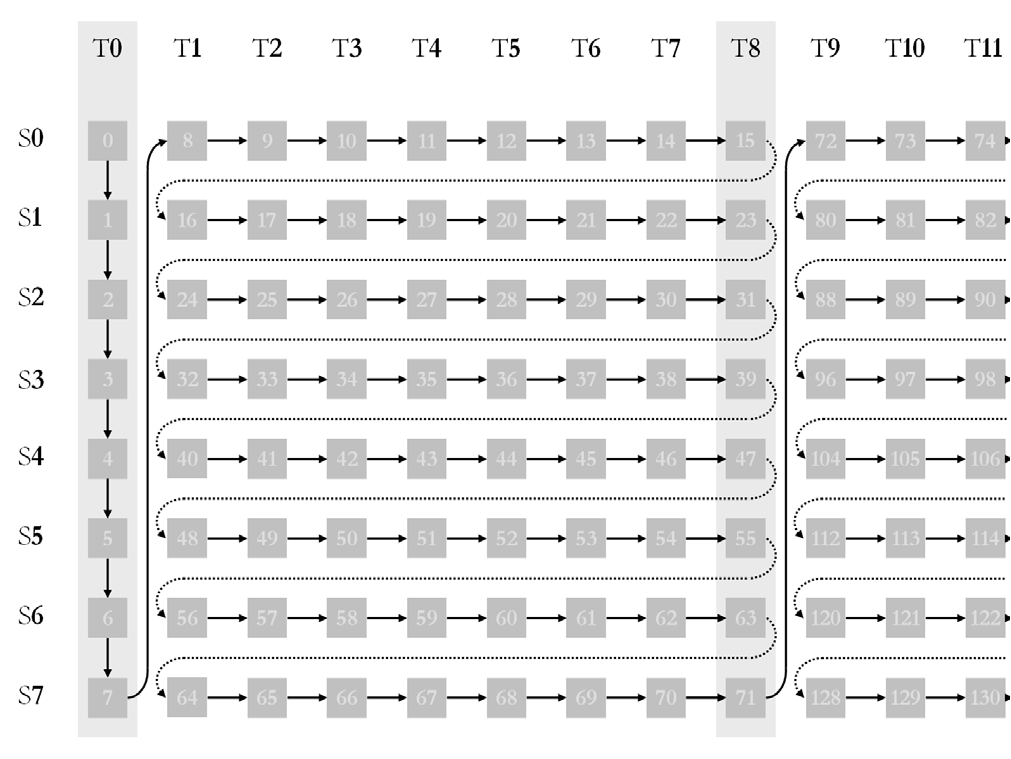
\includegraphics[width=7cm]{../img/encoding-memory}
\end{wrapfigure}

Die beschriebene Kodierungsmethode erlaubt es zudem eine effiziente Anordnung von Rahmen im Datenstrom.\cite{paper}
\texttt{T*} beschreibt hierbei den Zeitpunkt des Rahmens und \texttt{S*} die Perspektive.
Ein signifikanter Vorteil ist hier die Parallelisierung des Dekodierens.
Vor dem Zeitpunkt \texttt{T9} sind alle vorhergehenden Ansichten im Speicher geladen.
Die Ansichten h\"angen jeweils voneinander ab, aber es gibt hierbei immer Paare von ''Quellansichten'' und
''Senkenansichten''.
Die Quellansichten k\"onnen unabh\"angig voneinander dekodiert werden.

\noindent\\ Die Kodierungseffizienz ist hierbei stark abh\"angig von der Videosequenz.\cite{paper}
Im folgenden Diagramm sieht man einen Vergleich von \textit{Peak Signal to Noise Ratios} zwischen \textit{Simulcast}
und der \texttt{MVC}-Implementierung.
Die Variationen sind kein Mangel des Kodierungsverfahrens -welches im Schnitt immer noch eine Verbesserung gegen\"uber
Simulcast ist- vielmehr sind manche Videosequenzen schlichtweg nicht geeignet um per MVC kodiert zu werden.

\begin{center}
    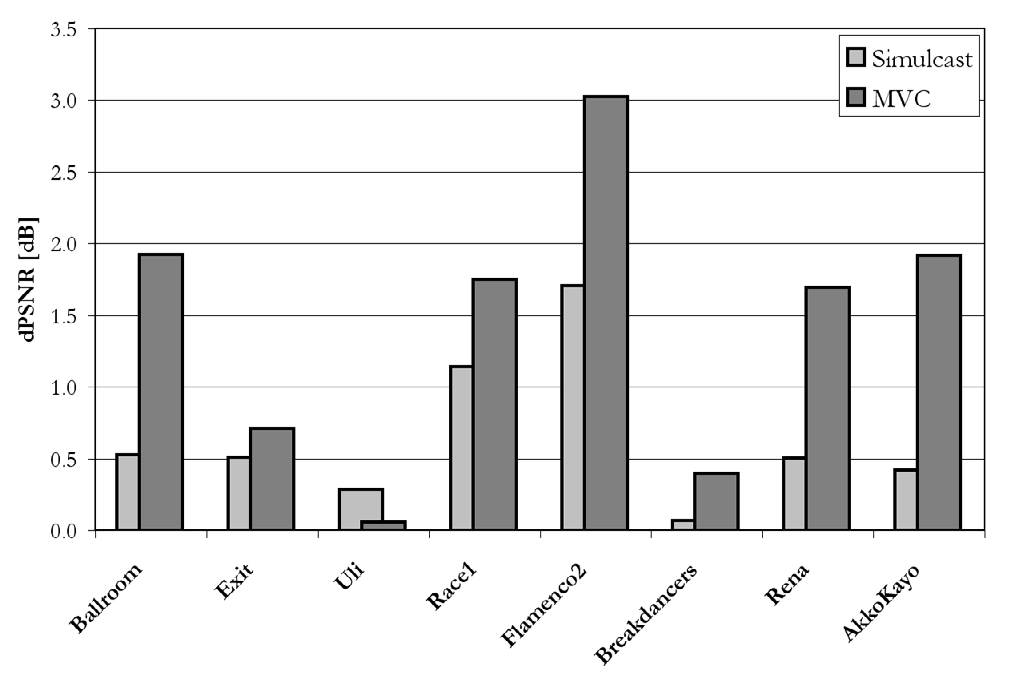
\includegraphics[width=0.75\textwidth]{../img/encoding-efficiency}
\end{center}
\noindent Ein triviales Beispiel hierf\"ur ware eine Sequenz, in welcher zwei 10 cm entfernte Kameras auf ein Objekt
gerichtet sind.
Eine davon ist allerdings auf einen Laternenpfahl gerichtet, an welchem die andere vorbeischaut.
Hierbei g\"abe es offensichtlich au{\ss}er der Lichtatmosph\"are des Bildes kaum Redundanzen.


    \pagebreak

    \section{Zusammenfassung}\label{sec:summary}
    \noindent\newline Das Kodieren von meherer Perspektiven (\textit{Multi-View-Coding}) und deren separates Darstellen ist
eine popul\"are Methode um den visuellen Effekt eines dredimensionalen Videos zu erzeugen.
Jedoch bringt dieses auch einzigartige Herausforderungen mit sich, da unsere Videosequenz um eine Raumachse erweitert
wird.

\noindent\newline Unter Nutzung von hierarchischen B-Rahmen-Baumstrukturen k\"onnen wir erfolgreich Multi-View-Coding
f\"ur \texttt{H.264} implementieren.
Unsere Implementierung ist sowohl f\"ur mehrere Perspektiven skalierbar als auch effizient im Speicher
anordenbar.
Zwar existieren Ausnahmef\"alle, jedoch sehen wir konsistente Reduktion in der Datenmenge im Vergleich
zu Simulcast.

\noindent\newline Die Flexibilit\"at des \texttt{H.264}-Codecs erlaubt es uns solche Baumstrukturen standardkonform
zu kodieren.
Bedauernswerterweise existiert au{\ss}er \texttt{FRIM}\cite{frim} keine Implementierung von \texttt{MVC}, insbesondere
\texttt{ffmpeg}\cite{ffmpeg} unterst\"utzt dies nicht.







    \pagebreak

    \addcontentsline{toc}{section}{\numberline{9} Literaturverzeichnis}
    \bibliographystyle{abbrv}
\begin{thebibliography}{9}
    \bibitem{random_digits}
    RAND:
    \textit{A Million Random Digits with 100,000 Normal Deviates} (1955)
    \\\texttt{\url{https://www.rand.org/content/dam/rand/pubs/monograph_reports/MR1418/MR1418.deviates.pdf}}
    (abgerufen 2019-06-01)

    \bibitem{ferranti_rng}
    A. M. Turing, R. A. Brooker:
    \textit{Programmer's Handbook for the Manchester Electronic Computer Mark II (2. Auflage)} 1. (1952)
    \\\texttt{\url{http://curation.cs.manchester.ac.uk/computer50/www.computer50.org/kgill/mark1/progman.html}}
    (abgerufen 2019-06-01)

    \bibitem{middle_square}
    Die 1949er Papiere wurden erst 1951 neu gedruckt:
    \\J. Neumann, Von:
    \textit{Various Techniques Used in Connection with Random Digits}
    (1951, National Bureau of Standards, Applied Math Series)
    \\\texttt{\url{https://mcnp.lanl.gov/pdf_files/nbs_vonneumann.pdf}}
    (abgerufen 2019-06-01)

    \bibitem{latexcompanion}
    W. Killmann, W. Schindler; Bundesamt f\"ur Sicherheit in der Informationstechnik:
    \textit{A proposal for Functionality classes for random number generators} (2011-09-18)
    \\\texttt{\url{https://www.bsi.bund.de/SharedDocs/Downloads/DE/BSI/Zertifizierung/Interpretationen/AIS_31_Functionality_classes_for_random_number_generators_e.pdf?__blob=publicationFile}}
    (abgerufen 2019-04-30)
    %Addison-Wesley, Reading, Massachusetts, 1993.

    \bibitem{seminumerical algorithms}
    D. E. Knuth:
    \textit{The Art of Computer Programming, Volume 2: Seminumerical Algorithms} (1997, Addison-Wesley)
    \\\texttt{\url{https://doc.lagout.org/science/0_Computer%20Science/2_Algorithms/The%20Art%20of%20Computer%20Programming%20%28vol.%202_%20Seminumerical%20Algorithms%29%20%283rd%20ed.%29%20%5BKnuth%201997-11-14%5D.pdf
    }}
    (abgerufen 2019-06-01)

    \bibitem{pokemon}
    ''Fractal Fusion'':
    \textit{Pokemon RBGY Random Number Generator}
    \\\texttt{\url{https://web.archive.org/web/20190105083840/http://tasvideos.org/GameResources/GBx/Pokemon.html}}
    (abgerufen 2019-06-01)

    \bibitem{fortran}
    Compaq:
    \textit{Compaq Fortran Language Reference Manual}
    \\\texttt{\url{http://h30266.www3.hpe.com/odl/unix/progtool/cf95au56/lrm0315.htm#randu_intrin}}
    (abgerufen 2019-05-04)

    \bibitem{neumann}
    J. Neumann, Von:
    \textit{Various techniques used in connection with random digits}, 12. 36-38
    (1951, National Bureau of Standards, Applied Mathematics Series)
    \\\texttt{\url{https://dornsifecms.usc.edu/assets/sites/520/docs/VonNeumann-ams12p36-38.pdf}}
    (abgerufen 2019-04-30)

    \bibitem{einstein}
    Frank Yellin et al. f\"ur Oracle:
    \textit{Random.java} (2014-03-04, OpenJDK)
    \\\texttt{\url{http://hg.openjdk.java.net/jdk8/jdk8/jdk/file/tip/src/share/classes/java/util/Random.java}}
    (abgerufen 2019-04-30)

    \bibitem{aes}
    N. Ferguson, B. Schneier, T. Kohno:
    \textit{Cryptography Engineering: Design Principles and Practical Applications} (2010, Wiley Publishing)
    \\\texttt{\url{https://www.schneier.com/academic/paperfiles/fortuna.pdf}}
    (abgerufen 2019-06-01)

\end{thebibliography}


\end{document}
